\documentclass[a4paper, 11pt]{article}
\title{Riemannov integral na pravokutniku i Fubinijev teorem}
\author{Magda Klari\'c}
\usepackage[croatian]{babel}
\usepackage[utf8]{inputenc}
\usepackage[T1]{fontenc}
\usepackage{lmodern}
\usepackage[text={16cm,24cm},centering]{geometry}

\usepackage{amssymb, amsmath, amsthm} % math stuff
\usepackage{listings, enumerate} % lists and enumerations

\usepackage{bigstrut}%tables

\usepackage{sagetex}

\usepackage{tikz}
\usepackage{pgfplots,wrapfig}

\usetikzlibrary{arrows,intersections,calc}
\usepackage{verbatim}



\theoremstyle{plain}
\newtheorem{definition}{Definicija}[section]
\theoremstyle{plain}
\newtheorem{theorem}[definition]{Teorem}
\newtheorem{proposition}[definition]{Propozicija}
\newtheorem{lemma}[definition]{Lema}
\newtheorem{corolar}[definition]{Korolar}

\theoremstyle{definition}
\newtheorem{example}[definition]{Primjer}

\theoremstyle{remark}
\newtheorem{remark}[definition]{Napomena}

\begin{document}
\maketitle


\newpage
\tableofcontents{}
\newpage

\section{Riemannov integral omeđene funkcije na pravokutniku}

Neka je $f:A=[a,b] \times [c,d] \to \mathbb{R} $ ograničena funkcija. Subdivizijom $P$ pravokutnika $A$ zvat ćemo izbor točaka 
$$
    a=x_0 < x_1 < \ldots < x_{n-1} < x_n =b; \quad \quad c=y_0 < y_1 < \ldots < y_{n-1} < y_n =d;
$$

\noindent Te točke određuju subdiviziju pravokutnika $A$ na $mn$ pravokutnika
$$
    A_{ij} = [x_{i-1}, x_i] \times [y_{j-1}, y_j], \quad i=1,\ldots, n;j=1,\ldots, m.
$$

Formalnije rečeno, subdivizija $P$ je uređen par subdivizija $P_{[a,b]}$ segmenta $[a,b]$ i $P_{[c,d]}$ 
segmenta $[c,d]: P=(P_{[a,b]},P_{[c,d]})$. 

Neka $m_{ij}, M_{ij}$ označavaju redom infimum i supremum funkcije f na pravokutniku $A_{ij}$. Donju i gornju Darbouxovu sumu pridruženu subdiviziji $P$ definiramo kao
\begin{align*}
    s&=s(P)=\sum_{i=1}^n \sum_{j=1}^m m_{ij}(x_i-x_{i-1})(y_j - y_{j-1}) \\
    S&=S(P)=\sum_{i=1}^n \sum_{j=1}^m M_{ij}x_i-x_{i-1})(y_j - y_{j-1})
\end{align*}

Budući da je $(x_i-x_{i-1})(y_j - y_{j-1})$ površina pravokutnika $A_{ij}$, te da je (u slučaju $f \leq 0\,) m_{ij}$ visina
upisanog kvadra iznad $A_{ij}$ i ispod grafa funkcije $f$, vidimo da je $s(P)$ volumen upisan
ispod grafa funkcije $f$ i iznad pravokutnika $A$. Taj je volumen (za integrabilnu funkciju $f$ i za
dovoljno finu subdiviziju $P$) aproksimacija odozdo za volumen ispod grafa funkcije $f$ i iznad
pravokutnika $A$. Analogno, $S(P)$ je opisani volumen grafu funkcije f iznad $A$, koji aproksimira
volumen ispod grafa i iznad $A$ odozgo.

Ako označimo sa $m$ odnosno $M$ infimum odnosno supremum funkcije $f$ na čitavom pravokutniku $A$,
onda očito za bilo koju particiju $P$ vrijedi
    $$
        m(b-a)(d-c) \leq s(P) \leq S(p) \leq M(b-a)(d-c)
    $$
\noindent
Slijedi da je skup svih donjih Darbouxovih suma ograničen, pa ima supremum. Skup svih gornjih
Darbouxovih suma je takoder ograničen pa ima infimum. Kažemo da je funkcija $f$ integrabilna
na $A$ ako je $\sup_P s(P) = \inf_P S(P)$. U tom slučaju taj broj nazivamo integralom funkcije $f$ po
$A$ i označavamo sa
    \begin{equation}\label{opcint}
        \int_A f= \sup_P s(P) = \inf_P S(P)
    \end{equation}
\noindent
Za \eqref{opcint} se koriste i oznake $\iint_A f$ ili $\iint_A f(x,y) dxdy$.\\
Sada možemo formulirati Lebesgueov teorem za funkcije 2 varijable. Za skup $S \subset \mathbb{R}^2$ kažemo da ima (Lebesgueovu) mjeru nula ako se za bilo koji $\varepsilon > 0$ skup $S$ može pokriti sa najviše prebrojivo mnogo otvorenih pravokutnika čija je ukupna površina (tj. suma njihovih površina) manja od $\varepsilon$.

    \begin{theorem}[\bf Lebesgue]
        Ograničena funkcija $f : A = [a,b] \times [c,d] \to \mathbb{R}$ integrabilna je na A
    (u Riemannovom smislu) ako i samo ako skup njezinih prekida $S$ ima (Lebesgueovu) mjeru nula.
    Posebno, svaka je neprekidna funkcija na $A$ integrabilna.

    \end{theorem}

Ovaj teorem rješava problem nalaženja primjera integrabilnih funkcija (pod uvjetom da dobro
razumijemo kada podskup od A ima mjeru 0). Ostaje pitanje računanja integrala. Ono je riješeno Fubinijevim teoremom koji nam je sljedeća tema.
    

\section{Fubinijev teorem}

Promotrimo sljedeći jednostavan primjer: neka je funkcija $f : A = [0, 1] \times [0, 2] \to \mathbb{R}$ dana sa
$f(x, y) = y$.\\


\begin{center}
\begin{sagesilent}
    x = var('x')
    y = var('y')
    step = .10
    x1 = 0
    x2 = 1.10
    y1 = 0
    y2 =2.10

    output = ""
    output += r"\begin{tikzpicture}[scale=1.0]"
    output += r"\begin{axis}[xmin=%d, xmax=%d, ymin=%d, ymax=%d,grid=major,grid style={dotted},colormap/greenyellow,shader=interp]"%(x1,x2,y1,y2-step)
    output += r"\addplot3[surf,mesh/rows=%d,mesh/cols=%d] coordinates {"%((y2-step-y1)/step+1,(x2-step-x1)/step+1 )
    # rows is the number of y values
    for y in srange(y1,y2,step):
        for x in srange(x1,x2,step):
            output += r"(%f, %f, %f) "%(x,y,y)

    output += r"};"
    output += r"\end{axis}"
    output += r"\end{tikzpicture}"
\end{sagesilent}
\sagestr{output}
\end{center}

\indent U ovom se primjeru integral može izračunati iz definicije \eqref{opcint} (učinite to, vidjet ćete da ne želite koristiti definiciju čak ni u jednostavnim slučajevima). Moguće je medutim uz pomoć slike
direktno odrediti volumen ispod grafa i iznad $A$, s obzirom da je riječ o prizmi, kojoj je baza
jednakokračni pravokutni trokut u $yz$ ravnini s katetama 2, i čija je visina jednaka 1. Dakle
    $$
    \int_A f= 2
    $$
S druge strane, izračunajmo “iterirani” integral
    \begin{equation*}
        \int_0^1 \left( \int_0^2y\, dy\right)\, dx= 
        \int_0^1 \left( \left.\frac{y^2}{2}\right\rvert^{y=2}_{y=0}\, \right)\, dx=
        \int_0^1 2\, dx= 
        \left.2x\right\rvert^{1}_{0}=
        2
    \end{equation*}
Iterirani integral u drugom poretku također daje isti rezultat:
    \begin{equation*}
        \int_0^2 \left( \int_0^1y\, dx\right)\, dy= 
        \int_0^2 \left( \left.yx\right\rvert^{x=1}_{x=0}\, \right)\, dy=
        \int_0^2 y\, dy= 
        \left.\frac{y^2}{2}\right\rvert^{2}_{0}=
        2
    \end{equation*}


    \begin{theorem}[\bf Fubini]
        Neka je $f : A = [a,b] \times [c,d] \to \mathbb{R}$ integrabilna funkcija. Pretpostavimo da je funkcija 
        sa $[c,d]$ u $\mathbb{R}$ dana sa $y \mapsto f(x,y)$ integrabilna na $[c,d]$ 
        za svaki (fiksirani) $x \in [a,b]$.
        Tada je funkcija $g :[a,b] \to \mathbb{R}$ dana sa
        $$
              g(x)=\int_c^d f(x,y)\, dy
        $$
        integrabilna na $[a,b]$ i vrijedi
        \begin{equation}\label{fub1}
            \int_A f=\int_a^b g(x)\, dx
            =\int_a^b \left(\int_c^d f(x,y)\, dy \right)\, dx.        
        \end{equation}
        Analogno, ako pretpostavimo da je funkcija sa $[a,b]$ u $\mathbb{R}$ dana sa $x \mapsto f(x,y)$ 
        integrabilna na $[a,b]$ za svaki (fiksirani) $y \in [c,d]$.
        Tada je funkcija $h :[c,d] \to \mathbb{R}$ dana sa $h(y)=\int_a^b f(x,y)\, dx$ integrabilna na $[c,d]$ i                 vrijedi
        $$
            \int_A f=\int_c^d h(y)\, dy
            =\int_c^d \left(\int_a^b f(x,y)\, dx \right)\, dy
        $$
    \end{theorem}

Primijetimo da su pretpostavke teorema očito ispunjene ako je $f$ neprekidna funkcija na $A$. Intuitivno, volumen ispod grafa funkcije $f \geq 0$ možemo podijeliti na “beskonačno tanke odreske” u smjeru $y$-osi. Volumen odreska kroz točku $x$ jednak je produktu površine $\int_c^d f(x,y)\, dy$ i debljine $dx$. To treba integrirati po $x$ da dobijemo čitav volumen.

Za (još jedan) primjer primjene Fubinijevog teorema, integrirajmo funkciju $f(x,y)= e^{2x+3y}$ po kvadratu $A=[0,1] \times [0,1]$:
\begin{center}
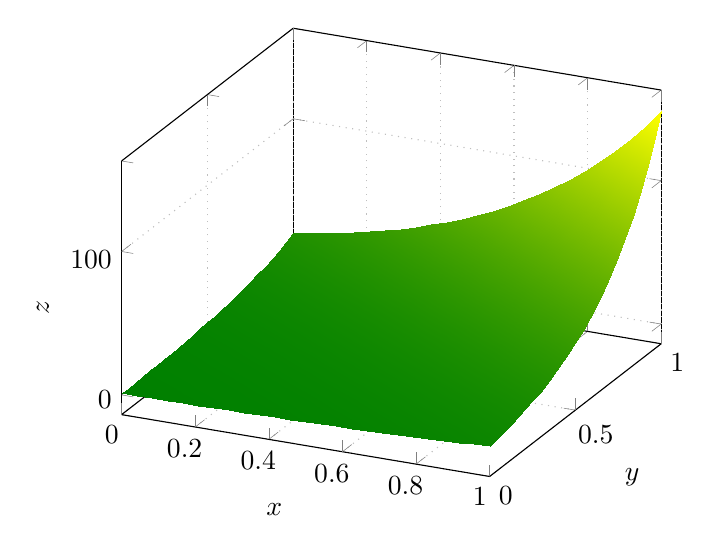
\begin{tikzpicture}[baseline]
\begin{axis}[colormap/greenyellow,
xlabel=$x$,ylabel=$y$,zlabel=$z$,
grid=major,grid style={dotted},shader=interp]
\addplot3[surf,domain=0:1] {exp(2*x+3*y)};
\end{axis}
\end{tikzpicture}
\end{center}

    \begin{multline*}
        \int_A f=
        \int_0^1 \left( \int_0^1 e^{2x+3y}\, dy\right)\, dx= 
        \int_0^1 \left( \left.\frac{1}{3}e^{2x+3y}\right\rvert^{y=1}_{y=0}\, \right)\, dx=\\
        \int_0^1 \frac{1}{3} \left( e^{2x+3}- e^{2x} \right)\, dx= 
        \frac{1}{6}\left.( e^{2x+3}- e^{2x})\right\rvert^{x=1}_{x=0} =
        \frac{1}{6}(e^5-e^3-e^2+1)
    \end{multline*}\newline

Za primjene nije dovoljno znati integrirati samo po pravokutnicima. 
Sljedeći korolar pokazuje kako integrirati po općenitijim područjima. 
Primijetimo prvo da se svaki ograničen skup $S \subset \mathbb{R}^2$ može pokriti nekim pravokutnikom $A$. 
Ako je  $f : C\to \mathbb{R}$ ograničena funkcija, proširimo je nulom do funkcije $\tilde{f} : A\to \mathbb{R}$ .
Tada kažemo da je $f$ integrabilna na $C$ ako je $\tilde{f}$ integrabilna na $A$ i definiramo
$$
    \int_C f= \int_A \tilde{f}
$$

S obzirom da je integral funkcije 0 jednak 0 po bilo kojem pravokutniku, lako se vidi da gornja
definicija ne ovisi o izboru pravokutnika $A$.

    \begin{corolar}
        Neka su $\phi, \psi :[a,b] \to \mathbb{R}$ neprekidne funkcije takve da je $\phi(x) \leq \psi(x)$ za svaka $x \in [a,b]$.
        Neka je $C$ područje u xy ravnini u pruzi $a \leq x \leq b$ i između grafova funkcija $\phi$ i $\psi$;
        drugim riječima, $(x,y) \in C$ ako i samo ako vrijedi $a \leq x \leq b$ i $\phi(x) \leq y \leq \psi(x)$.
        Neka je $f: C \to \mathbb{R}$ neprekidna funkcija. Tada je $f$ integrabilna na $C$ i vrijedi
        $$
            \int_c f=
            \int_a^b \left(\int_{\phi(x)}^{\psi(x)} f(x,y)\, dy\right)\, dx
        $$
    \end{corolar}
    
    \begin{proof}
    Pokrijmo $C$ pravokutnikom $A=[a,b] \times [c,d]$ i proširimo $f$ nulom do funkcije $\tilde{f} : A\to \mathbb{R}$.
    Tada je skup prekida funkcije $\tilde{f}$ sadržan u uniji grafova funkcija $\phi$ i $\psi$.
    Dakle Lebesgueov teorem povlači da je $f$ integrabilna na $C$ (odnosno da je $\tilde{f}$  integrabilna na $A$).\\
    Za fiksirani $x$, funkcija $y \mapsto \tilde{f}(x,y)$ je nula na $[c, \phi(x))$ i na $(\psi(x), d)$, a jednaka je $y \mapsto f(x,y)$
    dakle neprekidna je, na $[\phi(x), \psi(x)]$. Odavde odmah slijedi da je ta funkcija integrabilna na $[c, d]$
    i da vrijedi
        $$
            \int_c^d \tilde{f}(x,y)\, dy=
            \int_{\phi(x)}^{\psi(x)} f(x,y)\, dy
        $$

    Sada tvrdnja korolara slijedi direktno iz \eqref{fub1} Fubinijevog teorema.


\end{proof}


Dakako, moguće je zamijeniti ulogu varijabli x i y u korolaru pa integrirati neprekidne funkcije 
po području koje je u pruzi $c \leq y \leq d$ i između krivulja $x=\phi(y)$ i $x=\psi(y)$ 
gdje su $\phi$ i $\psi$ neprekidne funkcije sa $[c,d]$ u $\mathbb{R}$ 


\subsection{Neki primjeri}
\begin{example}
    Promotrimo integral $I=\displaystyle \int_0^1 \int_x^1 xy\,dydx$.\\
    Obratimo pažnju na skup $S=\{(x,y) \in \mathbb{R}^2 \mid 0 \leq x \leq 1,\, x \leq y \leq1\}$.
    Možemo primijetiti da je on jednak skupu $S'=\{(x,y) \in \mathbb{R}^2 \mid 0 \leq y \leq 1,\, 0 \leq x \leq y \}$
    
   \noindent Dakle možemo napraviti zamjenu poretka integrala i granica integriranja.
    
    \begin{sagesilent}
    x=var('x')
    y=var('y')
    dydxint = integral(integral(x*y,y,x,1),x,0,1) 
    dxdyint = integral(integral(x*y,x,0,y),y,0,1) 

    \end{sagesilent}
    
\begin{center}
     \renewcommand{\arraystretch}{2.5}
    \begin{tabular}{ c c c c c }
     Skup & $x$     & $y$    & integral                                   & rezultat \bigstrut[b] \\ \hline
     $S$ & $[0,1]$ & $[x,1]$ & $\displaystyle \int_0^1 \left( \int_x^1 xy dy\right)\,dx$ & $\sage{dydxint}$ \bigstrut \\ \hline
     
     $S'$& $[0,y]$ & $[0,1]$ & $\displaystyle \int_0^1 \left(\int_0^y xy dx\right)\,dy$ & $\sage{dydxint}$ \bigstrut[t]
    \end{tabular}
\end{center}
\end{example}
\noindent U prvom smo slučaju integrirali po varijabli y pa po varijabli x, a u drugom smo slučaju prvo integrirali po varijabli y pa onda po varijabli x.\newline

Zašto je u korolaru bitno da je $\phi(x) \leq \psi(x)$ za svaka $x \in [a,b]$? Promotrimo sljedeći primjer!

\begin{example}
    Neka je $\psi(x) =x$ i neka je $\phi(x)=1-x$ za $x \in [0,1]$.\\
    Površina skupa $S$ jednaka je $\int_S 1 dx$. 
   
   \begin{figure}[ht!]
    \centering
       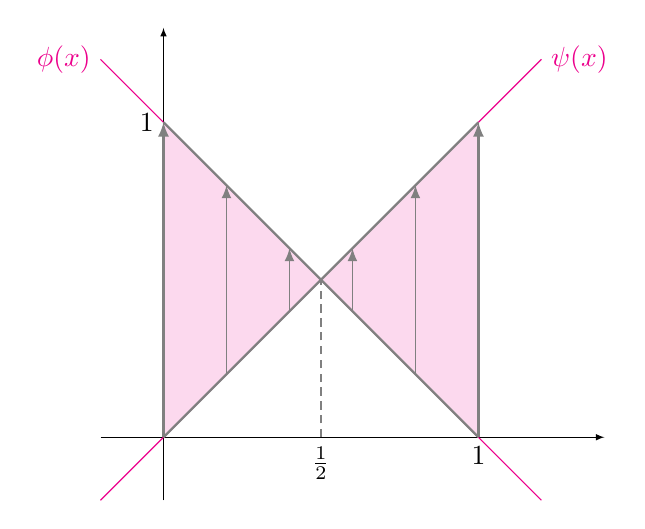
\begin{tikzpicture}[scale=4]
       \coordinate (x) at (1,1);
       \coordinate (y) at (0,1);
       \coordinate (z) at (1,0);
       \coordinate (S) at (0.5,0.5);   
       \coordinate (O) at (0,0);
       \draw (z) coordinate[label = {below:1}];
       \draw (y) coordinate[label = {left:1}];
       \draw (0.5,0) coordinate[label = {below:$\frac{1}{2}$}];

       \draw[>=latex,->,ultra thin] (-0.2,0)--(1.4,0) ;
       \draw[>=latex,->,ultra thin] (0,-0.2)--(0,1.3);;

       %psi i phi nacrtane
       \draw[magenta] (-0.2,-0.2) -- (1.2,1.2) coordinate[label = {right:$\psi(x)$}];
       \draw[magenta] (1.2,-0.2) -- (-0.2,1.2) coordinate[label = {left:$\phi(x)$}] ;

       %ispunjeno rozom
       \path[ fill =magenta!15] (O)--(S)--(y)--cycle;
       \path[ fill =magenta!15] (x)--(S)--(z)--cycle;

       %sive strelice 
       \draw[color=gray,>=latex,->,thick] (O)--(y);
       \draw[color=gray,>=latex,->,thick] (z)--(x);
       \draw[color=gray,>=latex,->,semithick] (0.2,0.2)--(0.2,0.8);
       \draw[color=gray,>=latex,->,semithick] (0.8,0.2)--(0.8,0.8);
       \draw[color=gray,>=latex,->,semithick] (0.4,0.4)--(0.4,0.6);
       \draw[color=gray,>=latex,->,semithick] (0.6,0.4)--(0.6,0.6);
       \draw[color=gray,thick] (O)--(x);
       \draw[color=gray,thick] (z)--(y);

       %iscrtkano
       \draw[color=gray,densely dashed] (0.5,0)--(S);

        \end{tikzpicture}
        \caption{Skup S}
     \end{figure}
    Sa slike 1. je jasno da to mora biti jednako 1/2.\\ 
    Računamo pripadni integral zanemarujući uvjet korolara:
    
    \begin{sagesilent}
    x=var('x')
    y=var('y')
    outerint = integral(integral(1,y,x,1-x),x,0,1) 
    \end{sagesilent}
    
    $$
        I=\int_0^1 \int_x^{1-x}1\,dydx= 
        \int_0^1 (1-x-x)\, dx=
        \int_0^1 (1-2x)\,dx=
        1-1= 0 =\text{(sage rezultat)}
        =\sage{outerint}
    $$
    što je očito pogrešno.
    Račun integrala primjenjujući korolar ide malo drukčije:
    $$
        \int_S 1\, dydx = 
        \int_0^\frac{1}{2} \int_x^{1-x}\,dydx+ \int_\frac{1}{2}^1 \int_{1-x}^x\,dydx= 
        \frac{1}{2}
    $$
\end{example}


Ovo je bio kratak uvod u Riemannov integral na pravokutniku. Za one koji žele znati više, preporučam predmet Integrali funkcija više varijabli!










\end{document}
